\documentclass[lettersize,journal]{IEEEtran}
\usepackage{amsmath,amsfonts}
\usepackage{xcolor}
\usepackage{pgfplots}
\pgfplotsset{compat=1.17}
\usepackage{tikz}
\usetikzlibrary{positioning}

\begin{document}

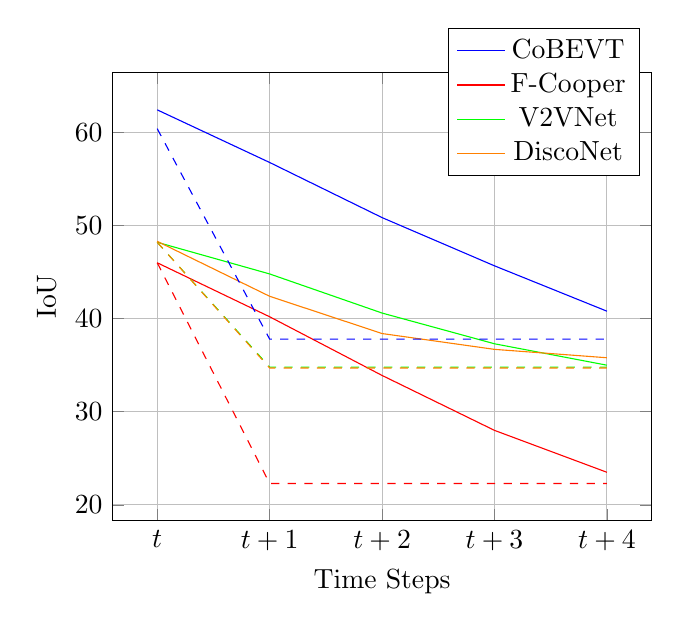
\begin{tikzpicture}
    \begin{axis}[
        xlabel={Time Steps},
        ylabel={IoU},
        xtick={1,2,3,4,5},
        xticklabels={$t$, $t+1$, $t+2$, $t+3$, $t+4$},
        ytick={10,20,...,70},
        % legend pos=north east,
        legend style={at={(0.8,1.1)},anchor=north},
        grid=both
    ]

    \addplot[color=blue,mark=none, solid] coordinates {
        (1,62.42) (2,56.77) (3,50.85) (4,45.67) (5,40.8)
    };
    \addlegendentry{CoBEVT}

    \addplot[color=red,mark=none, solid] coordinates {
        (1,46) (2,40.2) (3,33.9) (4,28) (5,23.5)
    };
    \addlegendentry{F-Cooper}

    \addplot[color=green,mark=none, solid] coordinates {
        (1,48.2) (2,44.8) (3,40.6) (4,37.3) (5,35)
    };
    \addlegendentry{V2VNet}

    \addplot[color=orange,mark=none, solid] coordinates {
        (1,48.3) (2,42.4) (3,38.4) (4,36.7) (5,35.8)
    };
    \addlegendentry{DiscoNet}


    % Dashed lines

    \addplot[color=blue,mark=none, dashed] coordinates {
        (1,60.4) (2,37.8) (3,37.8) (4,37.8) (5,37.8)
    };

    \addplot[color=red,mark=none, dashed] coordinates {
        (1,46) (2,22.3) (3,22.3) (4,22.3) (5,22.3)
    };

    \addplot[color=green,mark=none, dashed] coordinates {
        (1,48.2) (2,34.8) (3,34.8) (4,34.8) (5,34.8)
    };

    \addplot[color=orange,mark=none, dashed] coordinates {
        (1,48.2) (2,34.7) (3,34.7) (4,34.7) (5,34.7)
    };

    \end{axis}
\end{tikzpicture}

\end{document}